\section{Demarche Expérimentale}


\begin{minipage}{\textwidth}
    \begin{wrapfigure}{R}{0.5\textwidth}
        \centering
        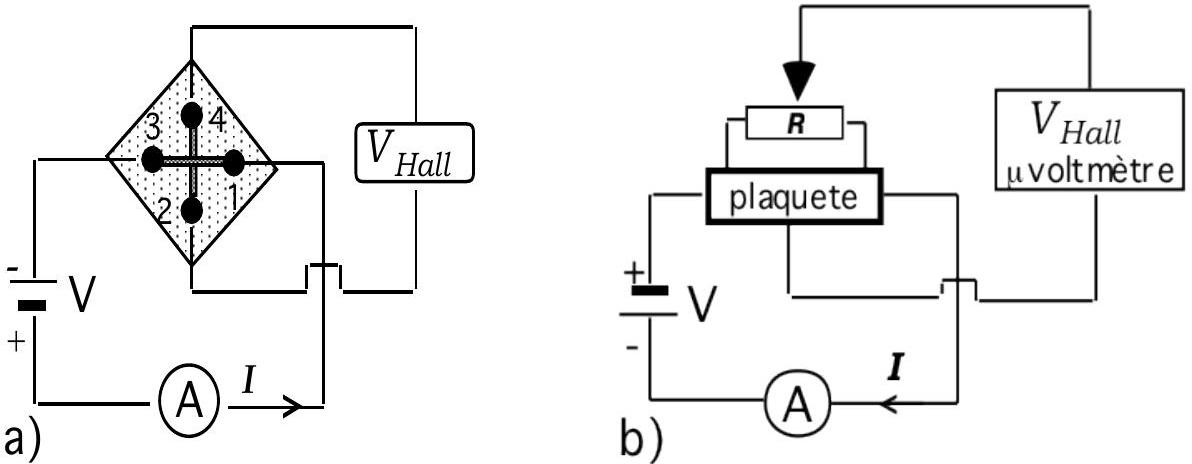
\includegraphics[width=\linewidth]{figures/montage.png}
        \caption{Dispositif expérimental utilisé pour constater l'effet Hall \cite{notice}}
        \label{fig:montage}
        \vspace*{1cm}
    \end{wrapfigure}

    Le montage expérimental utilisé dans cette expérience est composé de deux bobines en cuivre dans lequel un générateur permet de faire passer un courant continu créant ainsi un champ magnétique dans l'entrefer. Un échantillon peut être placé au niveau de celui-ci et ainsi permet de mesurer une tension de Hall quand un courant le traverse. Deux multimètre sont utilisés pour mesurer le courant entrant dans l'échantillon et pour mesurer la tension de Hall. La résistance interne du multimètre pris comme microvoltmètre est supposée suffisament grande pour ne pas affecter les mesures.
\end{minipage}

Les mesures du champ magnétique seront elles effectuées à l'aide d'un teslamètre qu'il convient de mettre à zéro avant le début des mesures. Il est important de ne pas trop faire bouger la tête de mesure durant son utilisation car l'intensité du champ magnétique mesurée dépend fortement de la position et de l'orientation.

\begin{minipage}{\textwidth}
    \begin{wrapfigure}{R}{0.5\textwidth}
        \centering
        \begin{subfigure}{0.25\textwidth}
            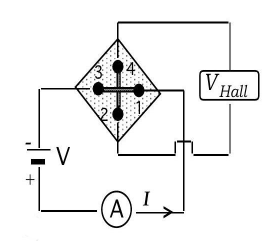
\includegraphics[width=\linewidth]{figures/circuit_4branch.png}
            \caption{}
            \label{fig:4branch}
        \end{subfigure}%
        \begin{subfigure}{0.25\textwidth}
            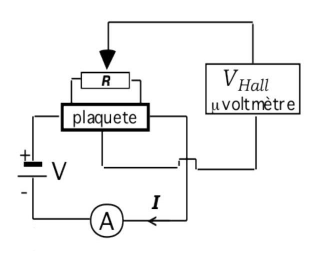
\includegraphics[width=\linewidth]{figures/circuit_5branch.png}
            \caption{}
            \label{fig:5branch}
        \end{subfigure}
        \caption{Méthodes de mesure de la tension de Hall à 4 contacts (a) et à 5 contacts (b) \cite{notice}}
        \label{fig:circuit}
        \vspace*{1cm}
    \end{wrapfigure}

    Afin de mesurer la tension de Hall deux types de branchements sont possibles. Le premier à 4 contacts \autoref{fig:4branch} permet de prendre plusieurs mesures aisément mais est affecté par une tension résiudelle présente même avec un champ magnétique nul. Le deuxième à 5 contacts \autoref{fig:5branch} dispose d'un potentiomètre branché en parallèle afin de se débarasser de cette tension résiduelle. Les mesures à 4 contacts ont été faites sur deux échantillons d'InP dopés au Si d'épaisseurs 1 \si{\micro\meter} et 2 \si{\micro\meter}. Les mesures à 5 contacts ont été faites sur un échantillon d'argent Ag d'épaisseur 1.9 \si{\micro \meter}, un de cuivre Cu d'épaisseur 1.6 \si{\micro \meter} et un de bismuth Bi d'épaisseur 3 \si{\milli \meter}.

    La détermination des valeurs de \(R_H\) et \(N\) peuvent se faire par la mesure de \(V_H\) en fonction de \(I\) ou de \(V_H\) en fonction de \(B\). Ces deux ensembles de mesures ont été effectués pour chaque échantillon.
    
\end{minipage}